\let\negmedspace\undefined
\let\negthickspace\undefined
\documentclass[journal]{IEEEtran}
\usepackage[a5paper, margin=10mm, onecolumn]{geometry}
%\usepackage{lmodern} % Ensure lmodern is loaded for pdflatex
\usepackage{tfrupee} % Include tfrupee package

\setlength{\headheight}{1cm} % Set the height of the header box
\setlength{\headsep}{0mm}     % Set the distance between the header box and the top of the text

\usepackage{gvv-book}
\usepackage{gvv}
\usepackage{cite}
\usepackage{amsmath,amssymb,amsfonts,amsthm}
\usepackage{algorithmic}
\usepackage{graphicx}
\usepackage{textcomp}
\usepackage{xcolor}
\usepackage{txfonts}
\usepackage{listings}
\usepackage{enumitem}
\usepackage{mathtools}
\usepackage{gensymb}
\usepackage{comment}
\usepackage[breaklinks=true]{hyperref}
\usepackage{tkz-euclide} 
\usepackage{listings}
% \usepackage{gvv}                                        
\def\inputGnumericTable{}                                 
\usepackage[latin1]{inputenc}                                
\usepackage{color}                                            
\usepackage{array}                                            
\usepackage{longtable}                                       
\usepackage{calc}                                             
\usepackage{multirow}                                         
\usepackage{hhline}                                           
\usepackage{ifthen}                                           
\usepackage{lscape}
\usepackage{circuitikz}



\author{EE25BTECH11041-Naman Kumar }
\graphicspath{./figs/}

\begin{document}
\begin{center}
    \huge{5.4.35}\\
    \large{EE25BTECH11041 - Naman Kumar}
\end{center}
Question:\\
Let p be an odd prime number and $\vec{T_p}$ be the following set of $2\times2$ matrices
\begin{align}
\vec{T_p}=\cbrak{\Vec{A}=\begin{pmatrix}a&b\\c&a\end{pmatrix}:a,b,c \in \cbrak{0,1,2,\dots,p-1} }
\end{align}
c) The number of A in $\vec{T}_p$ such that det(A) is not divisible by p is\\
\solution \\
\begin{align}
    det(\vec{A})=\begin{vmatrix}a&b\\c&a\end{vmatrix}\\
    =a^2-bc\\
\end{align}
Total number of possible matrices
\begin{align}
    =p\times p \times p=p^3
\end{align}
We can find number of matrices whose determinant is divisible by p\\
Required number = Total - number of matrices whose determinant is divisible by p
\begin{align}
    a^2-bc \equiv 0 \mod p \\
    a^2\equiv bc \mod p
\end{align}
Case 1: a=0
\begin{align}
    bc \equiv 0 \mod p
\end{align}
i) b=0, c as p-1 choices
\begin{align}
    \text{number of cases} = 1\times p=p
\end{align}
ii) c=0, b as p-1 choices
\begin{align}
    \text{number of cases} = 1\times p=p\\
    \text{total in this case}= 2(p)-1\label{1}
\end{align}
-1 for extra case of overlap at 'b' and 'c' both zero\\
Case 2: $a\neq0$\\
let $a^2=k$
\begin{align}
    \text{'a' has p-1 choices}\\
    bc \equiv k \mod p\\
    c\equiv k.b^{-1} \mod p \text{ ($b^{-1}$multiplicative inverse of b modulo p)}
\end{align}
For every 'b' we have a fixed 'c' for their are p-1 pairs of (b,c)
\begin{align}
    \text{number of cases}= (p-1)\times(p-1)=(p-1)^2 \label{2}
\end{align}
Finally adding total number cases from $\eqref{1}$ and $\eqref{2}$
\begin{align}
    =2p-1+(p^2-2p+1)
    =p^2 \label{3}
\end{align}
Finally required value is
\begin{align}
    \text{required ans}=total - \eqref{3}\\
    = p^3-p^2
\end{align}
\begin{figure}[H]
    \centering
    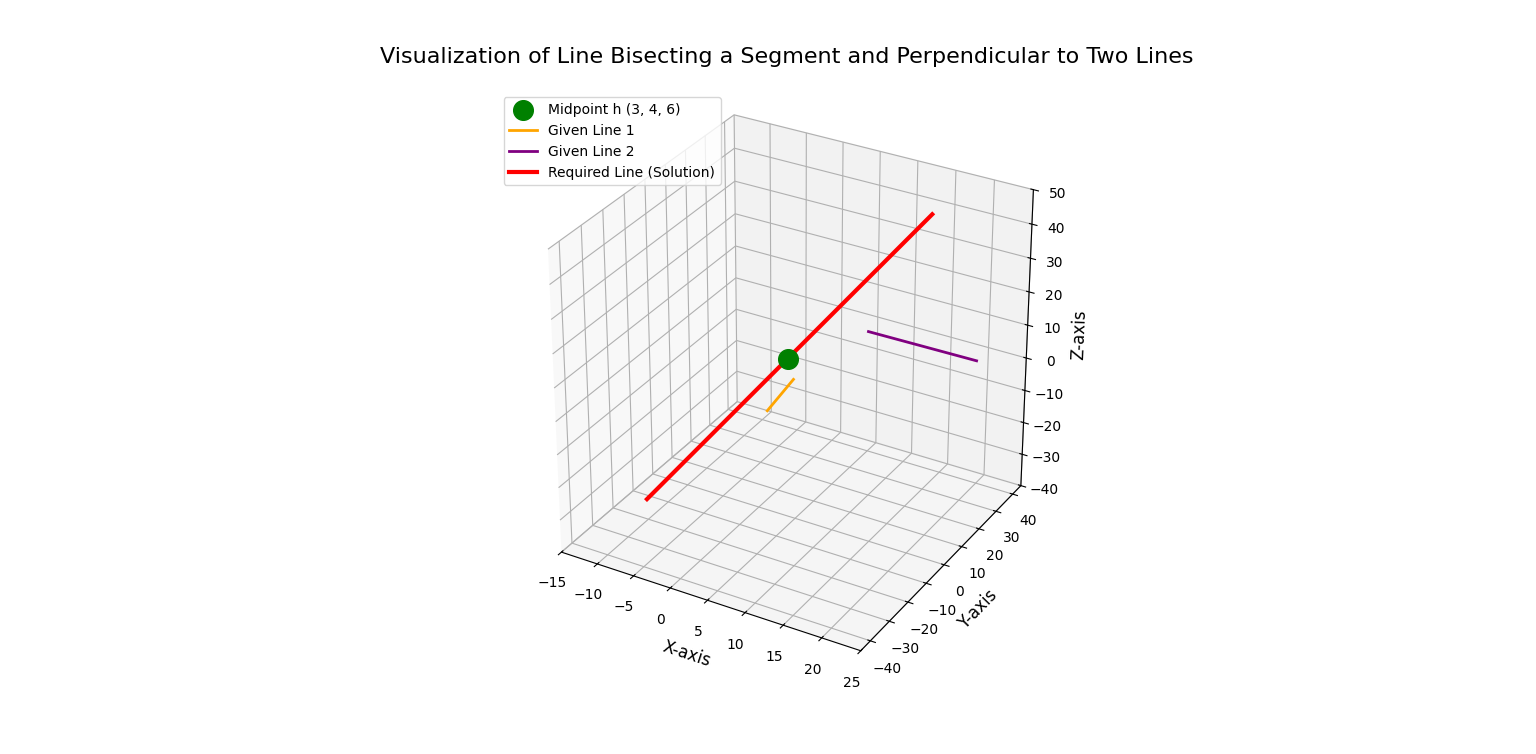
\includegraphics[width=\columnwidth]{figs/figure_c.png}
    \caption{}
    \label{fig:placeholder}
\end{figure}
\end{document}
